
\documentclass[11pt]{article}
\usepackage{acl2014}
\usepackage{times}
\usepackage{url}
\usepackage{latexsym}
\usepackage{graphicx}

\title{CS 288: Kneser-Ney Language Modeling}

\author{Anting Shen \\
  23566738 \\
  {\tt antingshen@berkeley.edu} \\
}
\date{September 12, 2014}

\begin{document}
\maketitle

\section{Introduction}

This report describes a Java implemenation of Kneser-Ney trigram language model, which estimates probability of a word type given the two preceding words. The model stores counts in optimized hashmaps and calculates probabilities at decode time. It is trained on a training corpus of nine million sentences, and tested as part of a machine translater. The model's implementation details, performance (BLEU, memory usage, decode speed), and areas for improvement follow.

\section{Smoothing Algorithm}

The algorithm used in this implementation is the unmodified Kneser-Ney described in Chen \& Goodman (1998), where $c(n-gram)$ is its count for $n=3$ and $|{w_i : count(w_i, ngram) > 0}|$ for $n=1$ and $n=2$. When the bigram being conditioned on has not been seen before, this language model reports the probability of the bigram model using fertilities instead of counts for simplicity, as it does not have a significant effect on BLEU. In the case that a type has not been seen before, the language model returns an arbitrary $0.000001$. The discount rate used is a constant 0.75, as it proved to have a better BLEU score than other tested discount rates. The variable discount rate from Chen \& Goodman's modified Kneser-Ney is not implemented.

\section{Data structures}

All types are asigned an integer during parsing to represent them in the language model to avoid storing strings. The language model is trained in one pass with no compression afterwards.

The fertilities (count of types that follow and count of types that precede) of unigrams, to calculate the base case of Kneser-Ney are stored in integer arrays indexed by the unigram. Since every unigram will have fertility counts, this method is dense, and occupies 4MB for all unigrams. The number of trigrams whose middle word is a given type is stored in this manner as well. Unigram counts are not stored as they are not needed for this version of Kneser-Ney.

Bigram \& trigram counts, as well as bigram fertilities, are stored in hashmaps keyed by a \texttt{long} calculated as the concatenation of the indices of the types in the ngram. Since Java hashmaps are inadequate in both memory and speed, custom counter classes are used. These counter classes are based on Carrot Search Labs OpenHashMap, and some methods such as hashing and expansion are copied.

The custom counters use Java primitive arrays for keys and data. A special key is used to denote empty slot. Keys are hashed using MurmurHash3, and are placed in the next slot in case of collision. For bigrams, counts and fertilities are stored in separate arrays of the same counter so keys are only stored once per bigram. The counter doubles in size when it reaches 75\% load. The counters only support incrementing by 1, and retrieving counts. When queries to the counter occur in pairs during decoding, such as fertility and count of bigrams, the counter fetches both and stores one in a cache instead of rehashing on the second query, which saves around 20\% decode time.

\section{Trading accuracy for memory}

Most counts in the trigram counter are very small and waste space as they are allotted 32 bits. In the training data, only around 150 trigrams appeared more than $2^{16}$ times. Because of this, I experimented with using 16-bit shorts to (no longer accurately) store trigram counts, and the results showed a 100MB reduction in memory usage. This was accompanies by a drop in BLEU from 24.8 to 24.7, which is a small amount to give up for the amount of memory saved. A small implementation was then tested to check for counter overflows and stop the counter at $2^{16}$ instead of overflowing, which would bring the counts closer to the actual count that the short was not capable of storing. However, this proved insignificant both in terms of additional decoding time to perform such check as well as BLEU, most likely due to some trigram counts reaching as high as around $2^{19}$, so using $2^{16}$ instead of a random short made little difference in the calculations.

The same modification was then made to the two bigram fertility counters as the two bigram fertility counters each had less than 50 overflows. Running the test with these modifications, there was another 50-100MB drop in memory use with no drop in BLEU. But when the bigram counts array was switched to shorts, the BLEU dropped to 23.5, which is an unacceptable tradeoff (despite still being above the cutoff). Nonetheless, these tweaks dropped printed memory usage to 1.0GB. 

\section{Additional potential improvements}

An alternate solution to overflowing the short would be to store an overflow bit as the highest bit of the counter. The overflowed bits would then be stored in the hashmap under the negative of the original key (since the sign bit is unused with $\le21$ bits per type in the trigram/bigram). This doubles the decode time and memory use of the ngrams that appear most frequently, but preserves the accuracy of the counter. Another implementation would be to store overflowed counts in a separate hashmap, and use the max short to signify overflow. The advantage of this method is that it allows 16 bits of counts before overflowing as opposed to 15.

More memory could also be saved by storing the bigram counts in the key array in the bigram counter. Since keys are of type \texttt{long}, and only 38 bits are needed to store the key. The only downside is code complexity and slight increase in decode time.

On the decode speed side, the language model is often queried for a small set of popular ngrams. Building a least-recently-used cache for these ngrams could greatly improve decode speed. The counters could also be processed and probabilities precomputed, though this would likely require more memory. 

\section{The biggest memory reduction...}

...turned out to be discarding training data. When all but 1.5 million sentences were discarded, the printed memory usage was a mere 341MB, yet BLEU remained as high as 24.419, suggesting that more data has only a small effect on BLEU, and that a much larger improvement can be gained from switching to Kneser-Ney trigram from a simple unigram LM (which is consistent with the Google paper, where algorithm choice made a large difference at small data sizes). However, this is a limited test case with a small corpus, so no real conclusions can be drawn. 

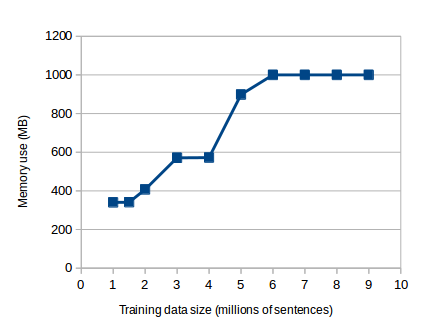
\includegraphics[keepaspectratio=true, width=220px, trim=17px 0px 0px 0px]{memory.png}

The above graph shows memory usage with the number of training sentences. Jumps are from hashmap resizing, and flat areas were increases in training data that did not trigger hashmap resizings.

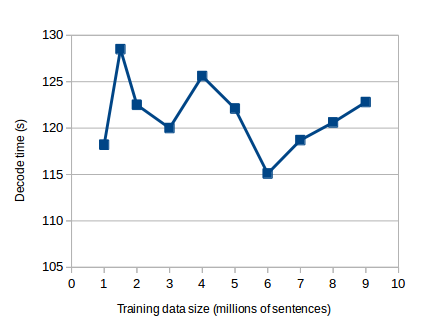
\includegraphics[keepaspectratio=true, width=220px]{decode.png}

The above graph here shows decode time, and as expected, the decode time increases when training data size increases and drops sharply when hashmap resizings are triggered, dropping the number of collisions. Though the variations were fairly insignificant compared to the unigram baseline of 6.22 seconds.

And most importantly, the BLEU score was measured for various training data sizes:

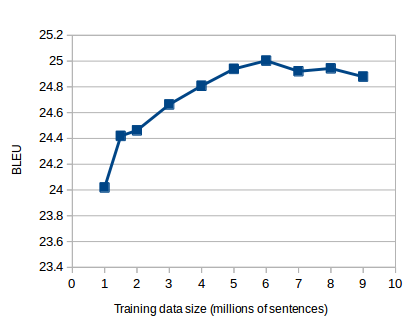
\includegraphics[keepaspectratio=true, width=220px]{bleu.png}

While translation quality improved with training data size, the improvement is small and had diminishing returns. This means that on a memory limited system, such as on a mobile device, one can get a large memory savings without sacrificing too much quality.

\section{Final results}

\begin{tabular}{| r | r | r |}
\hline
 & No discard & With discard \\ \hline
Training data size & 9 million & 1.5 million \\ \hline
Printed memory use & 1.0 G & 341 M \\ \hline
Decode time & 19.7x & 20.7x \\ \hline
BLEU & 24.879 & 24.419 \\ \hline
\end{tabular}
\end{document}
